\begin{enigme}[Un petit jeu de construction]

\begin{minipage}[c]{0.58\linewidth}
Comme cadeau de Noël, Zohra a eu un jeu avec des petites tiges aimantées et des boules métalliques. Au bout de chaque tige, on peut aimanter une autre tige ou une boule.
 \end{minipage} \hfill%
 \begin{minipage}[c]{0.38\linewidth}
  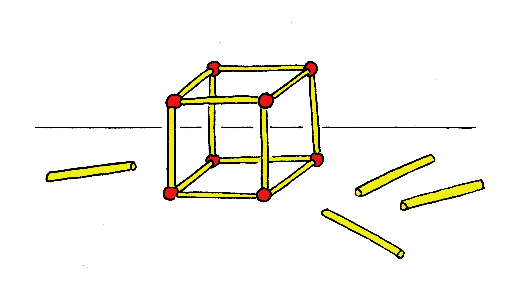
\includegraphics[width=5cm]{allumettes}
  \end{minipage} \\
Elle dispose de 48 tiges et de 8 boules. Elle cherche à construire, en utilisant tout ce matériel, le pavé droit le plus volumineux possible.
\begin{enumerate}
 \item Quels pavés droits peut‑elle construire ?
 \item Quel est celui qui a le plus grand volume ? Le plus petit volume ?
 \end{enumerate}

\end{enigme} 
